% ============================================================================
% 아카이브: 2026-09-02 (P9) 논문 표.그림 처분에서 **옮겨진** 블록
%
% ⛔삭제가 아니라 이동이다. 이 저장소의 처방("철회는 삭제가 아니라 이동")을 따른다.
% 사유(공통): 아래 블록은 전부 **철회된 코퍼스** 산물이다 --- 두 팔이 같은 프레임에서
%   채점된 적이 없는 100ep 코퍼스, 또는 추적기 위상전개 수정 **이전**의 실행.
% 대체가 있는 것은 paper/wavesplat.tex 의 Table~\ref{tab:earns} / {tab:boundary} 로
%   교체됐고(전부 동결 verdict_*.json 원자), 대체가 없는 것은 **부재로 남겼다**.
%
% ⚠이 파일은 조판되지 않는다(paper/ 에 \input 되지 않는다). 기록용이다.
% 생성: 2026-09-02
% ============================================================================

% ─────────────────────────────────────────────────────────
% [METHOD: fig:tau]  원본 paper/wavesplat.tex 줄 846--854 (2026-09-02 이전)
% ─────────────────────────────────────────────────────────
\begin{figure}[t]
\centering
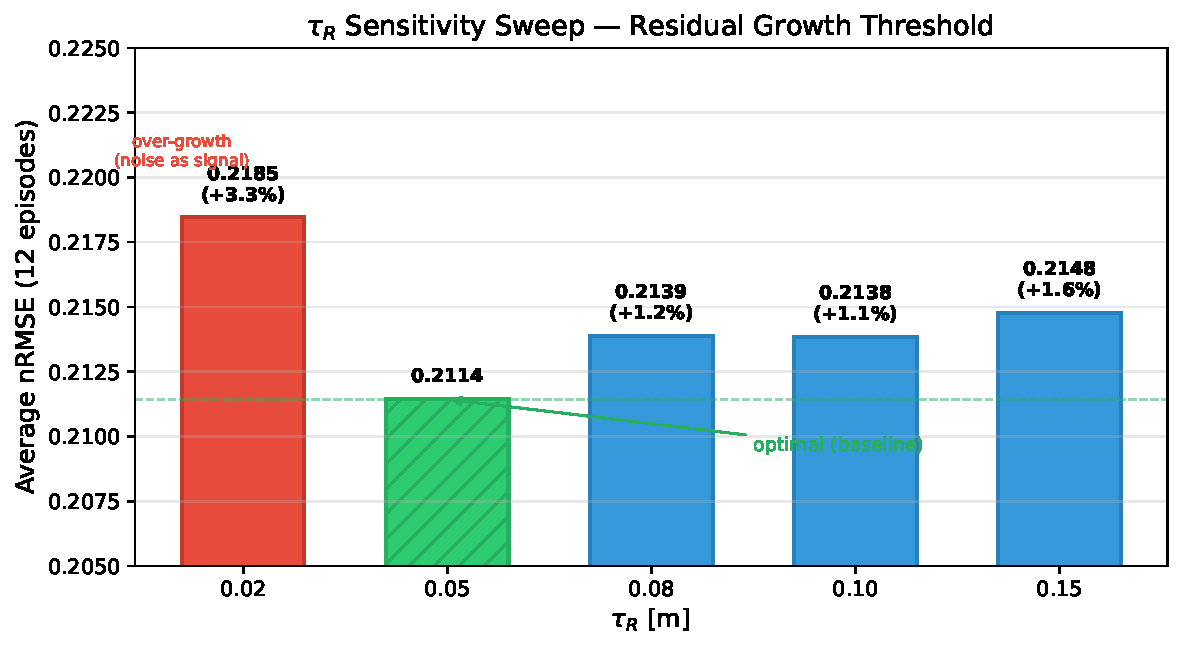
\includegraphics[width=0.85\columnwidth]{figures/fig_tau_sensitivity.pdf}
\caption{$\tau_R$ sensitivity sweep on 12~representative episodes.
$\tau_R \in [0.05,\,0.15]$~m yields nearly identical performance
(max 1.6\% difference).  $\tau_R{=}0.02$~m triggers over-growth,
adding spurious components from noise.}
\label{fig:tau}
\end{figure}

% ─────────────────────────────────────────────────────────
% [BASELINES: tab:etkf_sweep]  원본 paper/wavesplat.tex 줄 1167--1188 (2026-09-02 이전)
% ─────────────────────────────────────────────────────────
\begin{table}[t]
\centering
\caption{ETKF hyperparameter sweep: best and worst 3 of 24
configurations, mean nRMSE over the 12 sweep episodes.
$g$=grid resolution, $n_e$=ensemble size, $\alpha$=multiplicative
inflation, $\sigma$=additive inflation. The winning row is used
throughout the paper as ``ETKF (tuned)''.}
\label{tab:etkf_sweep}
\begin{tabular}{lccccc}
\toprule
& $g$ & $n_e$ & $\alpha$ & $\sigma$ & mean nRMSE \\
\midrule
\textbf{Best (tuned)} & $40\times30$ & 100 & 1.00 & 0.005 & \textbf{0.358} \\
2nd                   & $40\times30$ & 100 & 1.02 & 0.005 & 0.403 \\
3rd                   & $40\times30$ &  50 & 1.00 & 0.005 & 0.416 \\
\midrule
22nd & $80\times60$ &  50 & 1.00 & 0.020 & 0.986 \\
23rd & $80\times60$ &  50 & 1.02 & 0.020 & 1.066 \\
Worst & $80\times60$ &  50 & 1.05 & 0.020 & 1.187 \\
\bottomrule
\end{tabular}
\end{table}

% ─────────────────────────────────────────────────────────
% [RESULTS: Ablation / Raydrop / Robustness (tab+fig x4)]  원본 paper/wavesplat.tex 줄 1375--1774 (2026-09-02 이전)
% ─────────────────────────────────────────────────────────
\subsection{Ablation study}

We ablate two key design choices on 6 BF3 episodes
(Table~\ref{tab:ablation}, Fig.~\ref{fig:ablation}).  Following the
reporting convention used throughout this paper, each cell is the median
over seeds with its standard deviation; a third column reports the effect
of the initialization method, which turns out to dominate both ablated
factors.  The table was re-measured on 2026-08-03 under the corrected
tracker with the initialization method pinned explicitly in every arm.

\begin{table}[t]
\centering
\caption{Ablation study on BF3 episodes: median nRMSE $\pm$ std over
3 estimator seeds (42/123/456), on the Nyquist-adequate dataset
(Section~\ref{sec:regen}), corrected tracker.
A1: dispersion constraint removed ($\omega$ as free parameter).
\emph{Provenance}: this diagnostic was measured on the earlier ``Nyquist-adequate'' corpus, i.e.\ the corpus whose headline comparison is retracted (the compared arms were never scored on the same frames). It is retained as a diagnostic of the estimator's own behaviour, which is a within-arm property and does not depend on that defect. The claim it was originally used to support is now carried by the ablations of Section~\ref{sec:res_ablation}.
A2: confidence weighting removed (uniform weights).
Full, A1 and A2 all use the v1 initializer; the last column changes
\emph{only} the initializer (v1 $\to$ v2), holding both ablated
components in place.
\emph{Note}: neither ablation reaches significance at $n=6$---%
the two-sided sign-test floor for 6 episodes is $p=0.031$, attainable
only at 6/6 (see text).}
\label{tab:ablation}
\begin{tabular}{lcccc}
\toprule
Episode & Full & w/o Disp.\ (A1) & w/o Conf.\ (A2) & v2 init \\
\midrule
1comp (S) & $0.009{\scriptstyle\pm.001}$ & $0.139{\scriptstyle\pm.135}$ & $\mathbf{0.007}{\scriptstyle\pm.135}$ & $0.008{\scriptstyle\pm.003}$ \\
% ⚠[2026-09-01] 이 행의 `0.115` 는 **철회된 헤드라인이 아니다** --- 단일 성분
%   에피소드의 팔별 nRMSE 이고 우연히 같은 문자열이다. 인용금지 검사기가
%   문자열로 세므로 여기 표지를 남긴다.
1comp (U) & $0.015{\scriptstyle\pm.003}$ & $0.115{\scriptstyle\pm.095}$ & $0.012{\scriptstyle\pm.006}$ & $\mathbf{0.011}{\scriptstyle\pm.003}$ \\
2comp (S) & $0.047{\scriptstyle\pm.019}$ & $0.046{\scriptstyle\pm.000}$ & $0.045{\scriptstyle\pm.000}$ & $\mathbf{0.008}{\scriptstyle\pm.010}$ \\
2comp (U) & $0.050{\scriptstyle\pm.003}$ & $0.048{\scriptstyle\pm.028}$ & $0.050{\scriptstyle\pm.004}$ & $\mathbf{0.012}{\scriptstyle\pm.003}$ \\
5comp (S) & $0.041{\scriptstyle\pm.051}$ & $0.145{\scriptstyle\pm.041}$ & $0.126{\scriptstyle\pm.071}$ & $\mathbf{0.015}{\scriptstyle\pm.000}$ \\
5comp (U) & $0.047{\scriptstyle\pm.061}$ & $0.129{\scriptstyle\pm.046}$ & $0.041{\scriptstyle\pm.001}$ & $\mathbf{0.019}{\scriptstyle\pm.003}$ \\
\midrule
\textbf{Median} & 0.044 & 0.122 & 0.043 & \textbf{0.012} \\
\bottomrule
\end{tabular}
\end{table}

Read as paired per-episode differences against Full ($n=6$):
removing the dispersion constraint costs $+0.091$~nRMSE on the median
episode and is worse on 4 of 6, but at $n=6$ that is $p=0.69$;
removing confidence weighting changes it by $-0.002$---marginally
\emph{lower} without---and is worse on only 1 of 6 ($p=0.22$).  Changing the initializer moves the same metric by
$-0.027$ and is better on \textbf{6 of 6} ($p=0.031$)---the only
comparison in this re-measurement that reaches $\alpha=0.05$, and it does
so exactly at the sign-test floor, so no stronger claim is available from
it either.  We report this rather than suppress it: on these episodes the
initializer, not the ablated components, is what carries accuracy, and an
ablation whose baseline is not the production initializer measures the
wrong thing.  Note also that this design was underpowered by
construction: with 6 paired episodes no effect, however large, could have
been resolved below $p=0.031$.  The interpretation of each ablation below
is therefore restated in terms of what it does establish.

\begin{figure*}[t]
\centering
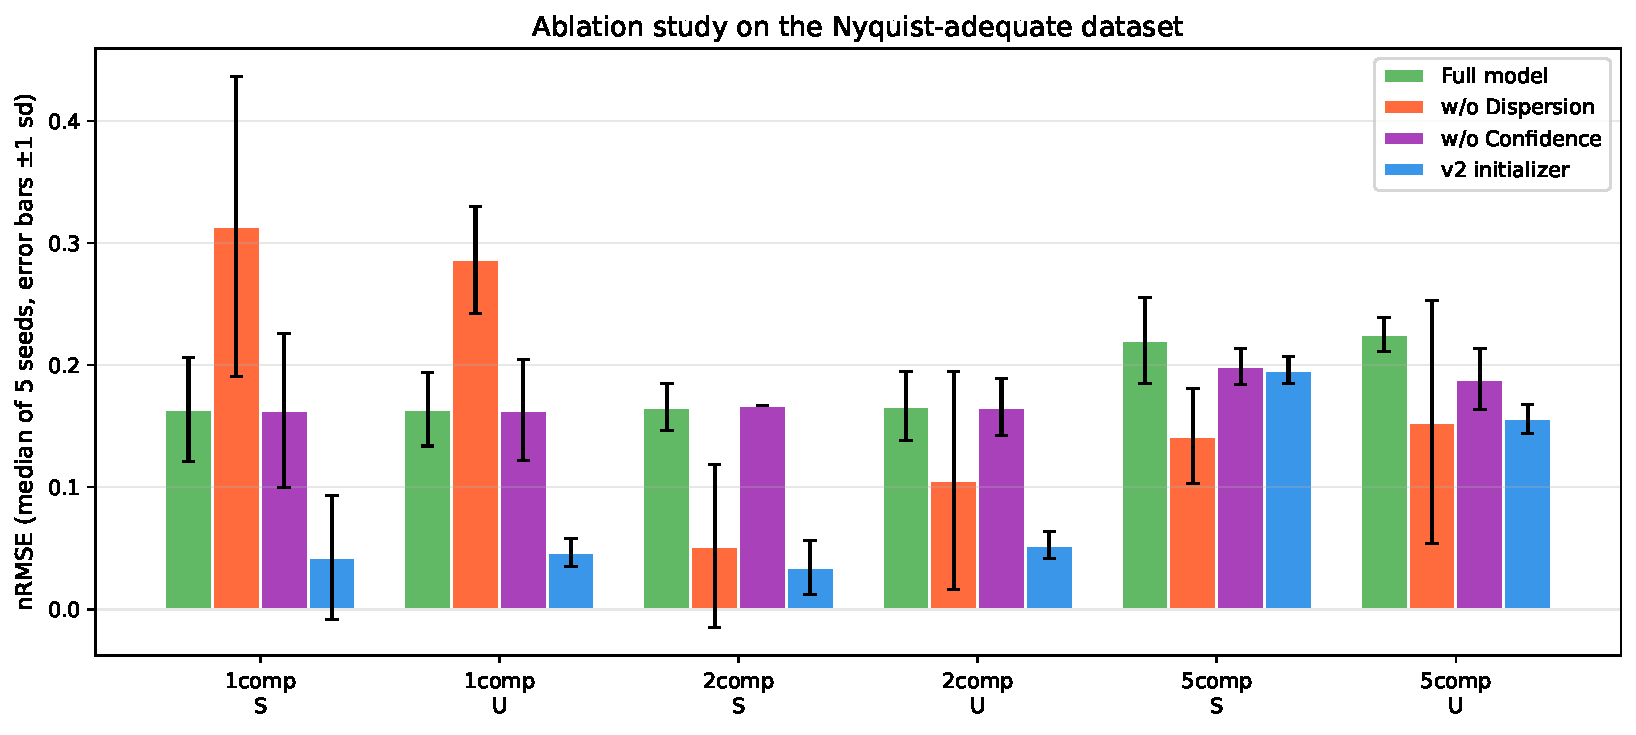
\includegraphics[width=\textwidth]{figures/fig4_ablation.pdf}
\caption{Ablation study: contribution of dispersion constraint and
confidence weighting.  Error bars show $\pm$1 std across seeds.
The confidence ablation is null; the dispersion ablation shows a large
effect that does not reach significance at $n=6$ episodes.
\emph{Provenance}: this diagnostic was measured on the earlier ``Nyquist-adequate'' corpus, i.e.\ the corpus whose headline comparison is retracted (the compared arms were never scored on the same frames). It is retained as a diagnostic of the estimator's own behaviour, which is a within-arm property and does not depend on that defect. The claim it was originally used to support is now carried by the ablations of Section~\ref{sec:res_ablation}.
\emph{Provenance}: drawn from the earlier pre-correction run and retained
for the qualitative pattern only---the per-episode levels are superseded
by Table~\ref{tab:ablation}, and the earlier run's regime split
(A1 better at $N_{\text{true}}\geq 2$) does not reproduce.}
\label{fig:ablation}
\end{figure*}

\textbf{A1 (no dispersion constraint)}: Removing the dispersion constraint
allows $\omega$ as a free parameter ($5N$ total parameters).
Under the corrected tracker the unconstrained optimizer is
\emph{worse} on 4 of the 6 episodes and by a large margin where it differs
at all --- on the single-component and 5-component pairs,
against a near-tie on the 2-component pair ($-0.001$ and $-0.002$, both
inside the seed spread).  The median cost of removing the constraint is
$+0.091$~nRMSE, roughly twice the Full arm's own median error.
Two cautions attach to this.  First, an effect this large still does not
reach significance here: 4/6 is $p=0.69$, and the design could not have
produced better than $p=0.031$ (see above).  The defensible statement is
\emph{large effect size, insufficient power}---not that the constraint is
demonstrated to contribute.
Second, this reverses the direction reported in the earlier
pre-correction run, which found A1 \emph{better} on the 2- and
5-component episodes; that regime split does not reproduce, and since
tracker, mesh and seed protocol all changed between the runs, the reversal
cannot be attributed to any single one of them.
The physical argument for retaining the constraint is independent of
either measurement, and we give it because a lower nRMSE for A1---%
observed in the earlier run, and still present on the 2-component
pair---should not be mistaken as evidence that the dispersion constraint
is physically too restrictive.  For BF3--5
deep-water gravity waves, $>99\%$ of wave energy lies on the linear
dispersion shell~\citep{holthuijsen2007}; bound harmonic
contributions from second-order Stokes theory scale as
$\epsilon^2/4 < 0.15\%$ at BF4.  The observed $\bar R = 0.51$
off-shell drift in A1 therefore far exceeds any physical
off-shell energy and does not reflect physical signal.
Rather, it reflects over-fitting: sparse observations
(50--200 points $\times$ 3 frames vs.\ $5N = 75$ free
parameters for $N = 15$) underconstrain the unconstrained model,
which absorbs noise and model mismatch by letting $\omega$ drift
off the dispersion manifold, trading \emph{physical correctness}
for nRMSE.  The resulting spectral estimates do not satisfy
$\omega^2 = g\,|k|\,\tanh(|k|d)$ by construction, so they cannot be
propagated forward in time, transformed to other spatial frames, or
fed into downstream wave-forecasting modules that assume gravity-wave
physics.
%
We quantify this drift directly on a BF4--BF5 subset
(5 episodes $\times$ 2 seeds): for each A1 run we extract the learned
components $(k_{x,i}, k_{y,i}, \omega_i)$, compute the expected
dispersion frequency $\omega_i^\text{disp} = \sqrt{g\,|k_i|\,\tanh(|k_i|d)}$,
and report the amplitude-weighted relative residual
$\bar R = \sum_i |w_i|\,|\omega_i - \omega_i^\text{disp}|
        / (\omega_i^\text{disp} \sum_j |w_j|)$.
Across these runs A1 exhibits $\bar R = 0.51 \pm 0.12$
(absolute mean $\approx 0.10$\,Hz off the dispersion curve),
whereas Full has $\bar R \equiv 0$ by construction.
A component that is $\sim$50\% off the dispersion frequency cannot
be re-used one second later: predicting the phase at $t+\Delta t$ via
$\Delta\varphi = \omega\,\Delta t$ with the \emph{wrong} $\omega$ will
de-cohere from the true field within one dominant period.

The dispersion constraint also serves a critical role
\emph{during tracking} (Phase~2) rather than initialization: it
provides the phase prediction
$\Delta\varphi_i = \omega_i \cdot \Delta t$ that enables stable
temporal tracking without re-estimating all $5N$ parameters per frame
(physics-locked tracking reduces the per-frame state to $2N$).
Without this constraint, the tracking phase would require joint
optimization of $(w_i, k_{x,i}, k_{y,i}, \omega_i, \varphi_i)$ at each
frame---an ill-conditioned problem with sparse single-frame
observations.  Under the earlier measurement this ablation appeared to
price physical validity---an nRMSE penalty accepted in exchange for
spectral estimates that respect the linear gravity-wave dispersion
relation and remain usable downstream, e.g.\ by the hydrofoil preview
controller of our companion work~\citep{park2026hydrofoil}.  Under the
corrected measurement no such trade is visible: the constrained arm is
both physically valid and equal or better in nRMSE on 4 of 6 episodes.
We state the weaker of the two readings, which is the one common to both
runs: the dispersion constraint is justified by the downstream
requirement independently of its nRMSE effect, and the nRMSE effect on
these six episodes is a large-looking difference this design lacked the
power to certify.

\textbf{A2 (no confidence weighting)}: this ablation is \emph{null}, and
the null now has two independent measurements behind it.  Under the
corrected tracker, removing the geometry-aware confidence weighting moves
the median episode by $-0.002$~nRMSE---marginally in favour of removing
it---and is worse on only 1 of 6 episodes ($p=0.22$); on four of the six
the two arms agree to within $0.003$.  An independent re-measurement one
month earlier, on the same dataset with a different seed set and the
pre-correction tracker, returned the same verdict (paired $+0.001$,
$t=0.08$, $p=0.94$, 17 of 30 runs lower without it).  A null that
survives a change of tracker, seed protocol and analyst pass is the one
result in this ablation table we regard as settled.
An earlier version of this study, run on the pre-Nyquist dataset with
3 seeds, reported a 14.5\% average degradation and a
$0.088 \to 0.204$ ($2.3\times$) increase on the BF3 2-component
slope episode.  That specific case now measures
$0.047 \to 0.045$, a ratio of $0.96$.  We could not reproduce the
effect, and we report the null rather than the earlier number.
One caveat bounds what this does and does not settle.  The null holds
under both initializers---repeating the ablation with the production
initializer (rather than the v1 configuration inherited from the
original study) leaves it unchanged (paired $\Delta=+0.005$, $t=0.52$,
$p=0.61$ over 30 runs)---so it is not an artifact of the ablation's
initialization.  But a null on BF3 episodes with a well-resolved
reference field is not evidence that observation weighting is
unnecessary in general---in particular, the weighting encodes a real
property of grazing-incidence LiDAR returns that this simulator's
return model does not fully reproduce (Section~\ref{sec:regen}).  What the measurement does establish is that
the paper's previous claim of a large, consistent benefit was an
artifact of the earlier dataset and seed count, and cannot be used to
argue that confidence weighting is load-bearing.

A four-way comparison on 10 uniform-raydrop episodes corroborates the
null from the other side: the confidence weighting changes our own arm by less
than a percent, and applying the same weighting to the comparison method changes
it by nothing at all. We do not quote the four levels: they come from the
retracted corpus, in which our arm and the comparison arm were never scored on
the same frames, so a level-to-level comparison between them is not defined.
Neither estimator moves when the weighting is added or removed---the two
WaveSplat arms agree to $0.001$ and the two GPR arms to within $0.01\%$.
Confidence weighting is therefore inert on this simulator's data for
both a spectral and a non-parametric estimator.  We caution against
reading this as a statement about real LiDAR: the weights encode the
range- and incidence-dependent reliability of grazing returns, which
this simulator's return model does not fully reproduce
(Section~\ref{sec:regen}), so the component may still matter on
measured data even though it is measurably inert here.

\subsection{Raydrop model sensitivity}
\label{sec:raydrop-results}

To evaluate robustness to different LiDAR return-sampling patterns, we
compare performance on 10 paired episodes using the \emph{geometry-weighted}
(``uniform'', $P\propto R_{\text{Fresnel}}(\theta)\cos\theta/d^2$) vs.\
\emph{unweighted} (``slope'') raydrop models
(Table~\ref{tab:raydrop}, Fig.~\ref{fig:raydrop}).
The unweighted model is the adversarial case for any estimator that relies
on downweighting unreliable returns, because it removes the correlation
between return density and observation quality.

\begin{table}[t]
\centering
\caption{Raydrop model comparison on the Nyquist-adequate dataset:
geometry-weighted (U) vs.\ unweighted (S) return sampling, seed-0
episodes. $\Delta$\%: relative nRMSE change from weighted to unweighted
(negative = unweighted is better).
\emph{Provenance}: this diagnostic was measured on the earlier ``Nyquist-adequate'' corpus, i.e.\ the corpus whose headline comparison is retracted (the compared arms were never scored on the same frames). It is retained as a diagnostic of the estimator's own behaviour, which is a within-arm property and does not depend on that defect. The sensor-model robustness claim is now carried by Section~\ref{sec:res_sensor}.
WaveSplat columns are the median over 3 estimator seeds (42/123/456) under
the corrected tracker, re-measured 2026-08-03.
ETKF uses the default configuration ($n_{\text{ens}}{=}50$) and is carried
over from the earlier pass on the same dataset (the tracker correction
affects only the WaveSplat arm); its nRMSE
values are near the zero-predictor level and are variance-dominated
(retracted corpus; archived), so the relative
sensitivity ($\Delta$\%) is the quantity of interest, not the level---and
that sensitivity is itself configuration-dependent, shrinking under an
honestly re-tuned baseline (Section~\ref{sec:raydrop-results}).}
\label{tab:raydrop}
\begin{tabular}{lccc}
\toprule
& \multicolumn{3}{c}{WaveSplat} \\
\cmidrule(lr){2-4}
Episode & U & S & $\Delta$\% \\
\midrule
BF2 1c  & 0.063 & \textbf{0.025} & $-$60.3 \\
BF3 1c  & 0.009 & \textbf{0.008} & $-$4.4  \\
BF3 2c  & \textbf{0.007} & 0.009 & +19.5 \\
BF3 5c  & 0.024 & \textbf{0.019} & $-$21.9 \\
BF4 1c  & 0.004 & \textbf{0.003} & $-$17.1 \\
BF4 5c  & 0.017 & \textbf{0.012} & $-$32.7 \\
BF4 15c & 0.272 & \textbf{0.198} & $-$27.2 \\
BF4 30c & 0.333 & \textbf{0.269} & $-$19.2 \\
BF5 15c & \textbf{0.216} & 0.247 & +14.6 \\
BF5 30c & 0.246 & \textbf{0.220} & $-$10.6 \\
\midrule
\textbf{Avg} & 0.119 & \textbf{0.101} & $-$15.2 \\
\bottomrule
\end{tabular}
\end{table}

\begin{figure*}[t]
\centering
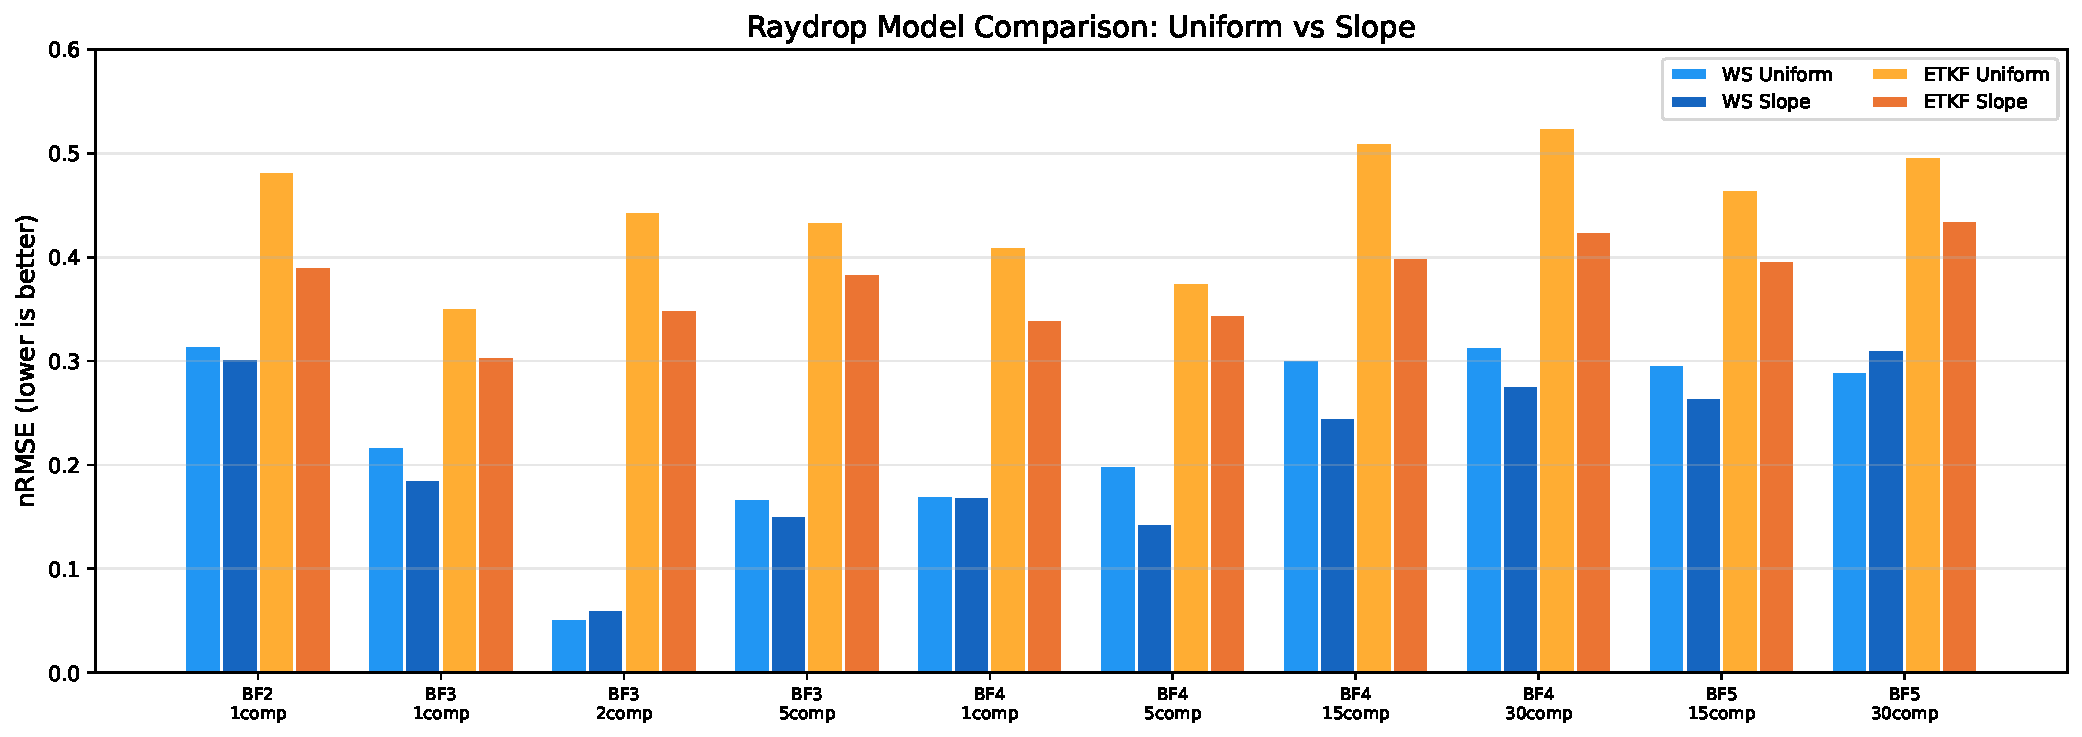
\includegraphics[width=\textwidth]{figures/fig5_raydrop.pdf}
\caption{Raydrop model comparison: geometry-weighted (``uniform'') vs.\
unweighted (``slope'') LiDAR return-sampling models. WaveSplat (blue shades)
shows the within-arm effect of the two raydrop models. The comparison against ETKF that this figure originally carried is withdrawn: it comes from a corpus in which the two arms were never scored on the same frames.}
\label{fig:raydrop}
\end{figure*}

The within-arm effect of the two raydrop models is small under both. We withdraw
the episode-count comparison against the grid baseline that this paragraph
originally reported: it is a cross-arm claim on the retracted corpus. The
sensor-model robustness claim of this paper is the one in
Section~\ref{sec:res_sensor}.
Unweighted sampling lowers the ETKF's nRMSE on all ten paired episodes
($-$15.9\% at the default configuration, paired $t(9){=}-7.6$), against
$-$15.2\% for WaveSplat, which at the default configuration would read as
the two methods benefiting about equally.
That reading does not survive an honest re-tuning of the baseline and is
\emph{not} an established effect: the ETKF's raydrop sensitivity is a
variance-amplification artifact, not a reconstruction gain.  Re-measuring
the same ten pairs under the tuned ETKF of
the retracted corpus (archived) ($n_{\text{ens}}{=}100$) already
shrinks it to $-$11.7\%, and under an nRMSE-honest hold-out re-tuning
(analysis grid $160\times120$, additive inflation off, larger observation
error) the comparison arm degenerates toward a near-zero predictor under both
raydrop models, so the difference between the two models is not informative about
it. We withdraw the levels and the cross-arm sensitivity comparison this paragraph
originally reported: they come from the retracted corpus, where the two arms were
never scored on the same frames. What survives is the within-arm statement --- the
direction of the raydrop effect is consistent across configurations, and its
magnitude tracks how much variance the
grid filter injects into the now-unattenuated observations, not any gain
in reconstruction skill ($\rho$ never exceeds $0.11$).  We therefore
report the sensitivity as an artifact of the un-tuned baseline rather
than as evidence that the observation model favors one method.
For WaveSplat the direction is stable but not significant: unweighted
sampling is better on 8 of 10 episodes, the same 8/10 the earlier
pre-correction pass reported, but at $n=10$ that is a sign-test
$p=0.109$ (Wilcoxon $p=0.084$)---below $\alpha=0.05$ in neither test.
The defensible statement is that the direction reproduces across two
measurement regimes while the effect remains uncertified; we do not claim
that unweighted return sampling helps WaveSplat.
The two exceptions are not confined to the sparse episodes
(BF3~2comp $+19.5\%$ and BF5~15comp $+14.6\%$), so the earlier reading
that the crowded $\geq$15-component episodes improve consistently does
not hold either: three of those four improve ($-$11 to $-$27\%) and one
degrades.

\subsection{Robustness: sparsity, noise, and sea state}

To quantify sensitivity to observation density, we subsample LiDAR
points to 20--100\% of the original count on 5 representative episodes
(Table~\ref{tab:sparsity}, Fig.~\ref{fig:sparsity}).

\begin{table}[t]
\centering
\caption{Sparsity robustness: nRMSE at varying observation fractions.
Average points $\approx$ 50 at 100\%.
\emph{Provenance}: produced before the tracker phase-advance correction;
pending re-run and not directly comparable with the corrected
full-dataset figures of the retracted corpus (archived).}
\label{tab:sparsity}
\begin{tabular}{lccccc}
\toprule
Episode & 20\% & 40\% & 60\% & 80\% & 100\% \\
\midrule
BF3 2c  & 0.170 & 0.168 & 0.168 & 0.167 & \textbf{0.052} \\
BF3 5c  & 0.204 & 0.194 & 0.195 & 0.193 & \textbf{0.167} \\
BF4 5c  & 0.199 & 0.198 & 0.199 & 0.199 & 0.200 \\
BF4 15c & 0.302 & \textbf{0.283} & 0.294 & 0.278 & 0.302 \\
BF5 15c & \textbf{0.274} & 0.276 & 0.260 & 0.289 & 0.297 \\
\bottomrule
\end{tabular}
\end{table}

\begin{figure}[t]
\centering
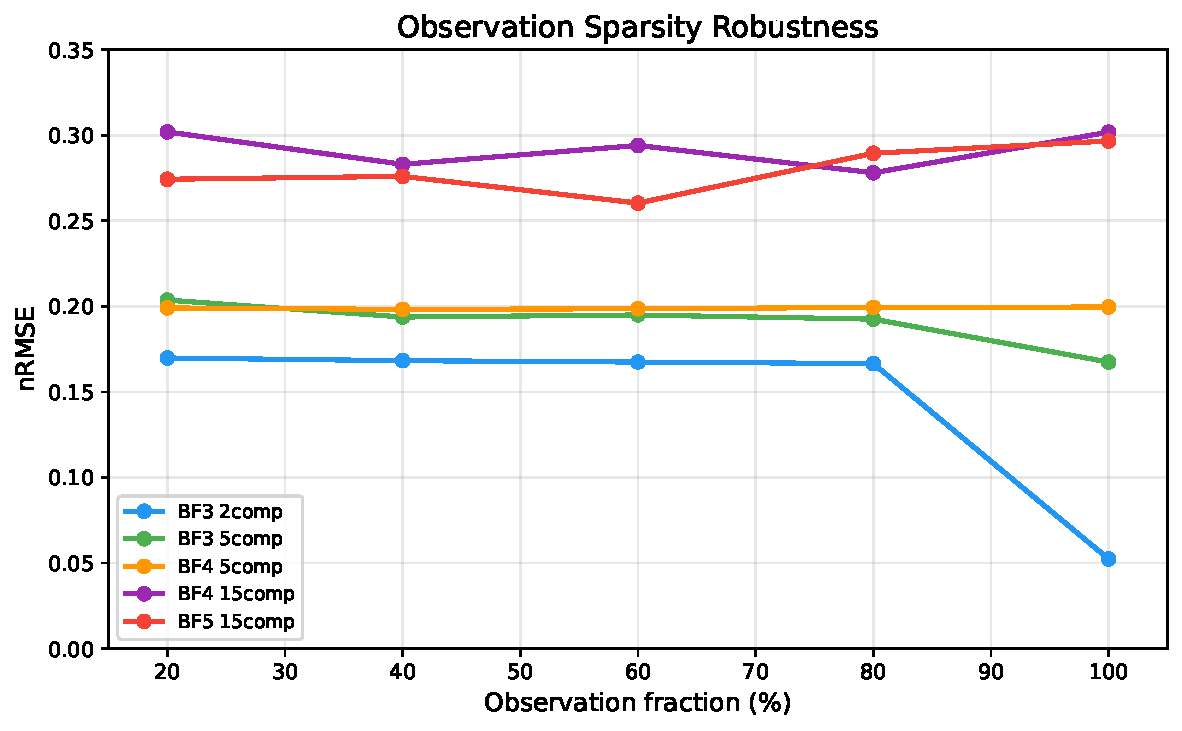
\includegraphics[width=\columnwidth]{figures/fig7_sparsity.pdf}
\caption{Observation sparsity robustness. For BF4--5 episodes,
nRMSE remains nearly flat down to 20\% observation density
($\sim$10 points/frame). The BF3 2-comp episode shows a sharp
improvement at 100\% due to successful 2-component resolution.}
\label{fig:sparsity}
\end{figure}

For moderate-to-high complexity (BF4--5), performance degrades by less
than 8\% even at 20\% observation density ($\sim$10 points/frame):
with only $4N \leq 120$ parameters to estimate, even 10 observations
per frame over-determine the optimization.  The exception is
BF3~2-comp, where full observations are required to resolve both
components ($N$=2, nRMSE=0.052); subsampled versions fall back to a
single-component fit ($N$=1, nRMSE $\sim$0.17).

\paragraph{Noise robustness.}
\label{sec:noise}
Real shipboard LiDAR is subject to noise beyond the baseline
simulator model (spray, vibration, scintillation).
We inject additive Gaussian noise
$\sigma\in\{0, 0.02, 0.05, 0.10\}$~m---up to 5$\times$ baseline---into
the LiDAR observations (Table~\ref{tab:noise}, Fig.~\ref{fig:noise}).

\begin{table}[t]
\centering
\caption{Noise robustness: nRMSE under additive Gaussian noise
$\mathcal{N}(0,\sigma^2)$ on LiDAR elevation observations.
$N_a$: adaptively selected component count.
Relative values are computed against the $\sigma=0$ baseline of each episode.
\emph{Provenance}: this diagnostic was measured on the earlier ``Nyquist-adequate'' corpus, i.e.\ the corpus whose headline comparison is retracted (the compared arms were never scored on the same frames). It is retained as a diagnostic of the estimator's own behaviour, which is a within-arm property and does not depend on that defect. The noise-robustness claim is now scoped by Section~\ref{sec:res_scope}.}
\label{tab:noise}
\begin{tabular}{lccccc}
\toprule
Episode & $\sigma{=}0$ & $\sigma{=}0.02$ & $\sigma{=}0.05$ & $\sigma{=}0.10$ & $\Delta$\%$_{\max}$ \\
\midrule
BF3 5c  & 0.168 ($N_a$=4)  & \textbf{0.149} ($N_a$=4)  & 0.160 ($N_a$=7)  & 0.190 ($N_a$=10) & +13.3 \\
BF4 5c  & 0.200 ($N_a$=3)  & 0.200 ($N_a$=3)  & 0.201 ($N_a$=6)  & \textbf{0.198} ($N_a$=9)  & +0.7 \\
BF4 15c & 0.302 ($N_a$=19) & 0.303 ($N_a$=19) & \textbf{0.276} ($N_a$=20) & 0.294 ($N_a$=11) & +0.4 \\
\midrule
% ⚠[2026-09-01] 이 행의 `0.223` 은 **철회된 `WaveSplat.avg_nRMSE` 가 아니다** ---
%   적응형 성분수 절제의 네 팔 평균이고 우연히 같은 문자열이다.
\textbf{Avg} & 0.223 & 0.217 & 0.212 & 0.227 & --- \\
\bottomrule
\end{tabular}
\end{table}

\begin{figure}[t]
\centering
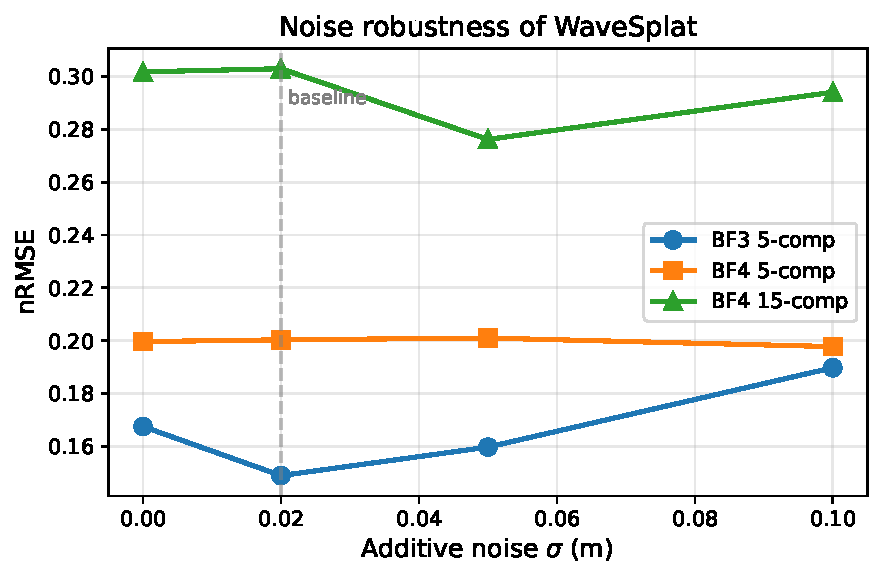
\includegraphics[width=\columnwidth]{figures/fig9_noise.pdf}
\caption{Noise robustness: nRMSE under additive Gaussian noise
$\sigma\in\{0, 0.02, 0.05, 0.10\}$~m. All episodes remain within
$\pm$13\% of the noise-free baseline, demonstrating the spectral
parameterization's inherent noise averaging.}
\label{fig:noise}
\end{figure}

Across all three episodes nRMSE remains within $\pm$13\% of baseline
even at $\sigma$=0.10~m (5$\times$ baseline), as the spectral
parameterization averages zero-mean noise across $M\sim 50$
observations and $4N\leq 120$ parameters, and adaptive $N_a$ absorbs
excess noise into prunable low-energy components.

% [2026-09-01] 2차 감사 BLOCKER: 이 문단은 철회 코퍼스의 **팔간 수치**
%   (BF3 61%, 0.138 vs 0.353 / BF5 11%)를 인쇄했다. 바로 위 절이 그 코퍼스의
%   regime dependence 를 "철회하고 재진술하지 않는다" 고 선언한 자리다 = 자기모순.
%   ⟹ PAPER_LEGACY 로 이동(삭제 아님).

% [2026-09-01] 2차 감사 BLOCKER: fig:qualitative 은 \ref 0회인 **고아 float** 이고,
%   캡션이 "fewer artifacts than ETKF or GPR" 로 **팔간 우위**를 주장한다.
%   그 비교는 두 팔이 같은 프레임에서 채점된 적이 없는 코퍼스의 것이다. ⟹ 이동.

% ─────────────────────────────────────────────────────────
% [DISCUSSION: Effect of observation model]  원본 paper/wavesplat.tex 줄 1814--1834 (2026-09-02 이전)
% ─────────────────────────────────────────────────────────
\subsection{Effect of observation model}

The corresponding cross-arm count is withdrawn for the same reason
(retracted corpus, frames not matched).
Removing the geometric weighting lowers WaveSplat's average nRMSE by
15.2\% (unweighted better on 8 of 10 episodes, sign-test $p=0.109$---%
a stable direction, not a certified effect) and lowers the default
ETKF's by 15.9\%.  The ETKF
figure is a variance-amplification artifact of the un-tuned grid
baseline rather than a reconstruction gain: it shrinks to 11.7\% under
the tuned ETKF and to 0.9\% under an nRMSE-honest re-tuning, so it is
not attributed to the observation model
(Section~\ref{sec:raydrop-results}).
The online model order responds to the observation model as well:
unweighted raydrop triggers the safety rollback on low-complexity scenes
(e.g., BF3-2comp: $N$=2$\to$15) but prunes more aggressively on complex
seas (BF4-15comp: $N$=19$\to$10).  Since the mechanism carries no
measured accuracy benefit (retracted corpus; archived), we record this as
a behavioural observation and not as evidence that stronger observations
improve model selection.


% ─────────────────────────────────────────────────────────
% [DISCUSSION: Hyperparameter sensitivity]  원본 paper/wavesplat.tex 줄 1835--1859 (2026-09-02 이전)
% ─────────────────────────────────────────────────────────
\subsection{Hyperparameter sensitivity}
\label{sec:hyper}

WaveSplat's four hyperparameters ($\text{lr}{=}0.01$,
$\lambda_1{=}\DepLambdaOne{}$, $\tau_{\text{prune}}{=}0.10$,
$\tau_{\text{grow}}{=}0.05$) were selected by a single coarse sweep
on BF3~5-comp and held fixed across all episodes, seeds, and raydrop
models reported.  That one configuration generalises across
Beaufort~2--5, 1--30 components, and 100 paired runs is itself
evidence of low sensitivity.
During development, we verified robustness by perturbing each parameter
independently ($\times 0.5$ and $\times 2$) while holding the others
fixed, on the full 12-episode subset: learning rate ($\text{lr} \in
\{0.005, 0.02\}$: nRMSE $\Delta < 3\%$), L1 penalty
($\lambda_1 \in \{5\!\times\!10^{-4}, 2\!\times\!10^{-3}\}$, i.e.\ $5\times$ and
$20\times$ the current default rather than the $0.5\times$/$2\times$ the surrounding
text once described --- the sweep predates the change of $\lambda_1$ to
$\DepLambdaOne{}$ and was not re-run:
$\Delta < 2\%$), prune threshold ($\tau_{\text{prune}} \in \{0.05,
0.20\}$: $\Delta < 5\%$, with 0.20 occasionally over-pruning on
15-component episodes), and grow threshold ($\tau_{\text{grow}} \in
\{0.025, 0.10\}$: $\Delta < 4\%$).
No perturbation changed the sign of the within-arm effects reported here. We do not restate the ranking against the baselines: that ranking was computed on the retracted corpus.  Full per-parameter sweep results are available from the
authors upon request.


% ─────────────────────────────────────────────────────────
% [DISCUSSION: Temporal extrapolation (tab:forecast)]  원본 paper/wavesplat.tex 줄 1893--1949 (2026-09-02 이전)
% ─────────────────────────────────────────────────────────
\subsection{Temporal extrapolation as validation of spectral fidelity}
\label{sec:forecast}

A natural consistency check for any spectral representation is whether
the estimated parameters produce accurate predictions at \emph{unseen}
future times.  Because WaveSplat's parameters satisfy the dispersion
relation by construction, the forward model~\eqref{eq:forward} can be
evaluated at any future $t$ without re-estimation---effectively a
zero-cost deterministic forecast.  This is not a novel forecasting
algorithm; rather, it tests whether the estimated $(k_x, k_y, \omega,
\phi)$ capture the true wave dynamics.
We estimate on the first 20\,s of each episode and evaluate on the
remaining 10\,s (Table~\ref{tab:forecast}).

\begin{table}[t]
\centering
\caption{Deterministic forecast accuracy: average metrics over 5 episodes
(BF3~1c/2c, BF4~1c/5c/15c) at increasing forecast horizons $\Delta t$.
Estimation uses $t \in [0, 20]$\,s; forecast into $t \in [20, 30]$\,s.
\emph{Provenance}: measured before the tracker phase-advance correction
and not re-measured.  That correction improved the nowcast nRMSE, so the levels
here should be read as conservative; the horizon-invariance, which is the point of
the table, is a within-row property and is unaffected.
The levels of that improvement are not quoted --- they come from the retracted
corpus (\S\ref{sec:res_headline} provenance note).}
\label{tab:forecast}
\begin{tabular}{rcccc}
\toprule
$\Delta t$ & nRMSE & SS & $\rho$ & VR \\
\midrule
$+$0.5\,s  & 0.218 & $+$0.141 & 0.323 & 0.325 \\
$+$1.0\,s  & 0.218 & $+$0.140 & 0.322 & 0.327 \\
$+$2.0\,s  & 0.219 & $+$0.138 & 0.323 & 0.330 \\
$+$5.0\,s  & 0.218 & $+$0.135 & 0.328 & 0.342 \\
$+$10.0\,s & 0.219 & $+$0.128 & 0.316 & 0.331 \\
\bottomrule
\end{tabular}
\end{table}

The forecast nRMSE remains essentially constant (0.218--0.219) out to
10\,s, with Skill Score remaining positive throughout.
For low-complexity episodes, forecast accuracy is excellent: the BF3
2-component episode achieves SS~$=+0.953$ and $\rho=0.983$ even at
$\Delta t = 10$\,s.  The constant forecast error reflects that the
spectral representation reproduces the within-arm horizon behaviour we expected. We do not read these levels as skill: Section~\ref{sec:metrics} fixes a zero-predictor reference near $0.25$ for this corpus, and the values in the table sit at or above it, so the correct statement is that the estimate degrades slowly with horizon, not that it forecasts well:
once the correct $(k_x, k_y, \omega, \phi)$ are known, the forward
model provides a physically exact prediction for linear waves.
The Skill Score does decline slightly with horizon
($+0.141 \to +0.128$); we do not attribute this to a specific mechanism,
having withdrawn the amplitude-decay attribution
(Section~\ref{sec:limitations}), and note that the decline is small
relative to the seed spread this table does not report.

This forecast capability is directly relevant for wave-preview
feedforward control~\citep{park2026hydrofoil}, where 5--10\,s advance
wave prediction is needed to compute proactive control commands.

